\documentclass[11pt,letterpaper]{article}
\usepackage[T1]{fontenc}
\usepackage[utf8]{inputenc}
\usepackage{amsmath,amsthm,mathtools}
\usepackage{newtxtext,newtxmath}
\usepackage[margin=1in,headheight=14pt]{geometry}
\usepackage{microtype}
\usepackage{graphicx,booktabs,array}
\usepackage{enumitem}
\usepackage{xcolor}
\usepackage{fancyhdr}
\usepackage[hidelinks,breaklinks]{hyperref}
\hypersetup{
 pdftitle={Sharp Conditioning Laws for Fabius and Lacunary Random Series},
 pdfauthor={AI-assisted research manuscript prepared for Vladimir Reshetnikov},
 pdfsubject={Full-configuration simplex coupling, sharp total-variation thresholds, and boundary phases},
 pdfkeywords={Fabius function, small deviations, Gibbs conditioning, lacunary series, total variation, Dirichlet distribution}
}
\usepackage{bookmark}
\usepackage{url}
\definecolor{heading}{HTML}{203B53}
\usepackage{titlesec}
\titleformat{\section}{\large\bfseries\color{heading}}{\thesection}{.7em}{}
\titleformat{\subsection}{\normalsize\bfseries\color{heading}}{\thesubsection}{.7em}{}
\pagestyle{fancy}
\fancyhf{}
\fancyhead[L]{\small Sharp conditioning laws}
\fancyhead[R]{\small Fabius and lacunary random series}
\fancyfoot[C]{\thepage}
\renewcommand{\headrulewidth}{.3pt}
\setlength{\parindent}{1.2em}
\setlength{\parskip}{3pt}
\setlength{\emergencystretch}{2em}
\setlist{itemsep=3pt,topsep=5pt}
\numberwithin{equation}{section}
\newtheorem{theorem}{Theorem}[section]
\newtheorem{lemma}[theorem]{Lemma}
\newtheorem{proposition}[theorem]{Proposition}
\newtheorem{corollary}[theorem]{Corollary}
\theoremstyle{definition}
\newtheorem{definition}[theorem]{Definition}
\newtheorem{remark}[theorem]{Remark}
\newcommand{\PP}{\mathbb P}
\newcommand{\EE}{\mathbb E}
\newcommand{\RR}{\mathbb R}
\newcommand{\NN}{\mathbb N}
\newcommand{\ZZ}{\mathbb Z}
\newcommand{\ind}{\mathbf 1}
\newcommand{\TV}{d_{\mathrm{TV}}}
\newcommand{\KL}{D_{\mathrm{KL}}}
\newcommand{\Law}{\mathcal L}
\newcommand{\Exp}{\operatorname{Exp}}
\newcommand{\Var}{\operatorname{Var}}
\newcommand{\Cov}{\operatorname{Cov}}
\newcommand{\Dir}{\operatorname{Dir}}
\newcommand{\Normal}{\mathcal N}
\newcommand{\eps}{\varepsilon}
\newcommand{\littleo}{o}
\newcommand{\Q}{Q_t}
\newcommand{\Px}{P_x}
\newcommand{\tQ}{\widetilde Q_t}
\newcommand{\tP}{\widetilde P_x}
\newcommand{\tD}{\widetilde D_t}
\newcommand{\rh}{\rho_n}
\newcommand{\vp}{\mathcal V}
\newcommand{\ip}{\mathcal I}
\DeclareMathOperator{\supp}{supp}
\DeclareMathOperator{\sgn}{sgn}

\title{\vspace{-1.1em}\textbf{Sharp Conditioning Laws for\break Fabius and Lacunary Random Series}\\[.55em]
\large A global simplex approximation, exact total-variation thresholds,\\
and phase-dependent boundary layers}
\author{\normalsize Research manuscript prepared for Vladimir Reshetnikov\\
\small AI-assisted derivations, with reproducible numerical checks}
\date{September 28, 2026}

\begin{document}
\maketitle
\thispagestyle{empty}
\begin{abstract}
Let $S=\sum_{j\ge1}w_jU_j$, where the $U_j$ are independent uniforms on $[0,1]$
and $0<w_{j+1}\le q w_j$ for a fixed $q<1$. We investigate the entire configuration
conditioned on $S\le x$, as $x\downarrow0$. Write $t$ for the exponential-tilting
parameter whose tilted mean is $x$, and $n=\#\{j:tw_j\ge1\}$. We prove a
quantitative approximation, in total variation on the full countable product
space, by independent Dirichlet proportions, the tilted tail, and an exponential
slack, followed by a common radial rescaling. Its error is
$O_q((1+\log\log n)/n)$.

For an arbitrary, possibly infinite coordinate set containing a proportion
$\alpha$ of the active coordinates, the distance between its conditioned and
tilted laws tends to
$\TV(\Normal(0,1-\alpha),\Normal(0,1))$. Thus negligible tilted variance is
exactly the criterion for asymptotic independence from the constraint.
For $k=o(n)$ growing bulk coordinates, the distance is
$\varphi(1)k/n+o(k/n)$; an explicit $L^1$ density expansion also gives fixed-coordinate
mean and covariance corrections. We obtain a Brownian-bridge limit, exponential
endpoint slack, Gumbel extremes, and an explicitly phase-dependent microscopic
boundary law for geometric weights. The dyadic case is the Fabius distribution.

The finite-i.i.d.	otal-variation phenomenon belongs to classical work of
Diaconis--Freedman. The contribution developed here is its quantitative
infinite-lacunary extension, especially the full-configuration approximation
and the simultaneous control of bulk, slack, and boundary. These are
manuscript proofs, not Lean-certified results; priority beyond the inspected
sources is not asserted.
\end{abstract}
\vfill
\noindent\textbf{Repository anchor.}\quad
\href{https://github.com/VladimirReshetnikov/ProveIt}{\texttt{VladimirReshetnikov/ProveIt}},
\texttt{Analysis/FabiusFunction}.\\
\textbf{Inspected snapshot.}\quad
{\small\texttt{2cdcd74f3abcbbff7bd47c6c4265522395def609}}.
\newpage
\tableofcontents
\newpage

\section{Research target, provenance, and scope}
\label{sec:scope}

The probabilistic construction of the Fabius function asks about the small
values of
\begin{equation}
 S_2=\sum_{j\ge1}2^{-j}U_j,\qquad F_2(x)=\PP(S_2\le x).
 \label{eq:fabius}
\end{equation}
This representation is classical; Arias de Reyna's Theorem~3 gives it in the
normalization $F_2(x)=\mathrm{up}(x-1)$ for $0\le x\le1$
\cite{arias}. The question studied here is not only \emph{how unlikely} $S_2\le x$
is, but \emph{what the infinitely many summands look like when that event occurs}.

The inspected ProveIt asymptotic audit reports an all-orders small-argument
expansion, with an exact Lambert phase and periodic correction terms
\cite{repo}. We do not re-prove that expansion or claim to have rebuilt its
Lean files. Instead we address three related questions. How many summands may
be inspected before the conditioning becomes statistically detectable? Can
one approximate the \emph{entire} conditioned configuration without making an
incorrect independence assertion? Where do the geometric oscillations survive
in a probabilistic limit?

Theorems below answer these questions for every uniformly lacunary sequence,
not just powers of two. The main mechanism is simple to state but requires
uniform error control: sufficiently early tilted summands are nearly
exponentials; their proportions form a simplex; and the remaining coordinates
have only $O(\log\log n)$ total tilted variance after a suitable split.

\subsection{What is classical, and what is being extended}

Diaconis and Freedman studied conditional laws of finite i.i.d.
exponential-family samples and obtained sharp variation asymptotics for both
$k/n\to0$ and proportional blocks \cite{df}. In particular, a linear $k/n$
threshold and a Gaussian proportional-block profile must not be advertised
as new finite-sample principles. We derive the needed simplex formulas
explicitly, with our convention $\TV=\tfrac12 L^1$, and extend them to an
infinite, non-identically distributed, increasingly tilted array.

Cator and Ferrari's more recent Gibbs-conditioning theorem concerns
independent nonnegative integer-valued log-concave laws, a fixed tilt, and weak
convergence under an anti-condensation hypothesis \cite{cf}. Our variables are
continuous, the tilt diverges, the event is a shrinking small ball, and the
main approximation is on a full countable product in total variation. This
comparison identifies different hypotheses and conclusions; it is not a
claim that existing general conditioning theory cannot also be adapted.

The repository review was targeted: its root map, Fabius asymptotic audit,
and narrow code searches were inspected. It was not an exhaustive reading of
every repository manuscript, nor an exhaustive priority search. Accordingly,
we describe the results as a proved manuscript-level extension and a candidate
contribution to this research program, not as a certified historical
breakthrough or a resolution of a named, published open conjecture.

\subsection{Conventions and proof organization}

For probability measures on the same measurable space,
\[
 \TV(P,Q)=\sup_A|P(A)-Q(A)|
 =\frac12\int\left|\frac{dP}{dQ}-1\right|dQ
 \quad(P\ll Q),
 \qquad
 \KL(P\Vert Q)=\int\log\frac{dP}{dQ}\,dP.
\]
Products over countably many coordinates carry the product Borel
$\sigma$-field. All limits are as $x\downarrow0$, equivalently $t\to\infty$.
Constants with a subscript $q$ may depend on the fixed lacunarity bound but
not on the particular weights, the observed coordinate set, or $t$, once $n$
is sufficiently large. The normal density and distribution function are
$\varphi$ and $\Phi$.

Sections~\ref{sec:setup}--\ref{sec:global} prove the full-configuration theorem.
Sections~\ref{sec:likelihood}--\ref{sec:mask} establish sharp marginal and
information-theoretic consequences. Sections~\ref{sec:process}--\ref{sec:extreme}
handle processes and extremes. The numerical checks and open research agenda
are separated from the proofs.

\section{The tilted array and its effective dimension}
\label{sec:setup}

Assume throughout that
\begin{equation}
 w_j>0,\qquad w_{j+1}\le q w_j\quad(j\ge1),\qquad 0<q<1.
 \tag{L}\label{eq:lacunary}
\end{equation}
No lower bound on $w_{j+1}/w_j$ is imposed. Thus very large gaps are allowed.
Let $P$ be the original product law and put
\[
 S=\sum_{j\ge1}w_jU_j,\quad F(x)=P(S\le x),\quad
 L(t)=\EE_P e^{-tS}=
 \prod_{j\ge1}\frac{1-e^{-tw_j}}{tw_j}.
\]
The series is bounded by $\sum_jw_j<\infty$, so these definitions pose no
integrability difficulty. For $0<x<\EE_PS$ there is a unique $t>0$ satisfying
\begin{equation}
 x=\EE_{Q_t}S,\qquad
 \frac{dQ_t}{dP}=\frac{e^{-tS}}{L(t)}.
 \label{eq:tilt}
\end{equation}
Indeed, the tilted mean is continuous, its derivative is
$-\Var_{Q_t}(S)<0$, its value at zero is $\EE_PS$, and it tends to zero.
The last assertion follows by dominated convergence coordinate by coordinate,
using summability of the weights. Also $F(x)>0$: choose a deterministic tail
bound below $x/2$, and then restrict finitely many uniforms to sufficiently
small positive intervals.

Define scaled coordinates, their caps, and the active dimension by
\begin{equation}
 Y_j=tw_jU_j,\quad a_j=tw_j,\quad
 T=\sum_{j\ge1}Y_j,\quad
 \mu=tx=\EE_{Q_t}T,\quad
 n=\#\{j:a_j\ge1\}.
 \label{eq:coordinates}
\end{equation}
The number $n$ is finite for fixed $t$ and tends to infinity with $t$.
Under $Q_t$ the coordinates are independent, with densities
\begin{equation}
 p_a(y)=\frac{e^{-y}}{1-e^{-a}}\ind_{(0,a)}(y),\qquad
 m(a)=1-\frac{a}{e^a-1},\qquad
 v(a)=1-\frac{a^2e^a}{(e^a-1)^2}.
 \label{eq:truncexp}
\end{equation}
Here $m$ and $v$ are the mean and variance. Their values near zero are understood
by continuous extension; in particular $m(a)=a/2+O(a^2)$ and
$v(a)=a^2/12+O(a^4)$.

\begin{lemma}[Active-dimension estimates]
\label{lem:dimension}
Uniformly under \eqref{eq:lacunary},
\begin{equation}
 \mu=n+O_q(1),\qquad V:=\Var_{Q_t}(T)=n+O_q(1).
 \label{eq:muV}
\end{equation}
Moreover, uniformly for every coordinate set $I\subseteq\NN$,
\begin{equation}
 \sum_{j\in I}v(a_j)=|I\cap[1,n]|+O_q(1).
 \label{eq:maskvar}
\end{equation}
\end{lemma}
\begin{proof}
For $r\ge0$, $a_{n-r}\ge q^{-r}$, whereas for $r\ge1$,
$a_{n+r}<q^{r-1}$. The active mean deficits $1-m(a)$ and variance deficits
$1-v(a)$ are nonnegative and decay exponentially in $a$ up to polynomial
factors. Their sums are bounded by convergent series evaluated at $q^{-r}$.
For the inactive tail, $0\le m(a)\le a$ and $0\le v(a)\le a^2$, so its
mean and variance sums are bounded by geometric series. This proves
\eqref{eq:muV}. The same argument bounds the sum of absolute discrepancies
$\sum_j|v(a_j)-\ind_{j\le n}|$ by a constant; restricting the sum to any $I$
gives \eqref{eq:maskvar}.
\end{proof}

Let $P_x=P(\,\cdot\mid S\le x)$ and define its nonnegative slack by
\begin{equation}
 H=\mu-T=t(x-S).
 \label{eq:slack}
\end{equation}
The exact change of measure is
\begin{equation}
 \frac{dP_x}{dQ_t}=
 \frac{e^{T-\mu}\ind_{\{T\le\mu\}}}{D_t},\qquad
 D_t=\EE_{Q_t}\big[e^{T-\mu}\ind_{\{T\le\mu\}}\big],\qquad
 F(x)=L(t)e^\mu D_t.
 \label{eq:weight}
\end{equation}
The weight in the numerator is at most one. This elementary fact will allow
an exponentially accurate product approximation to survive conditioning on
an event whose tilted normalizing mass is only of order $n^{-1/2}$.

\section{Separating an exponential bulk from the tail}
\label{sec:split}

For all sufficiently large $n$, set
\begin{equation}
 \ell=\left\lceil\frac{\log(6\log n)}{\log(1/q)}\right\rceil,
 \qquad N=n-\ell,\qquad
 \rho_n=\frac{\ell+1}{n}.
 \label{eq:cutoff}
\end{equation}
Then $\ell=O_q(1+\log\log n)$, $N\ge n/2$ eventually, and
$a_N\ge6\log n$. Write
\begin{equation}
 Z=(Y_j)_{j>N},\quad R=\sum_{j>N}Y_j,\quad r=\EE_{Q_t}R,\quad
 W=R-r,\quad
 \eps=\sum_{j\le N}(1-m(a_j)).
 \label{eq:taildef}
\end{equation}
In particular,
\begin{equation}
 \mu=N-\eps+r.
 \label{eq:muexact}
\end{equation}

\begin{lemma}[Tail moments and removable caps]
\label{lem:tail}
The above quantities satisfy
\begin{align}
 r+\EE W^2&=O_q(\ell+1),&
 \EE W^4&=O_q((\ell+1)^2), \label{eq:tailmoments}\\
 \eps&=O_q((\log n)n^{-6}),&
 \delta:=\sum_{j\le N}e^{-a_j}&=O_q(n^{-6}).
 \label{eq:caperror}
\end{align}
For each fixed even integer $p$, $\EE|W|^p=O_{q,p}((\ell+1)^{p/2})$.
\end{lemma}
\begin{proof}
There are $\ell$ remaining active coordinates. For $a\ge1$, the density
$p_a$ is bounded by $(1-e^{-1})^{-1}e^{-y}$, and hence every fixed raw or
centered moment is uniformly bounded. For $j>n$, the cap is bounded by a
geometric sequence, so the sums of all fixed positive powers of the caps
are bounded. This gives the mean and variance estimates.

For independent centered variables $X_j$, direct expansion gives
\[
 \EE\Big(\sum_jX_j\Big)^4
 =\sum_j\EE X_j^4+6\sum_{i<j}\EE X_i^2\EE X_j^2.
\]
The first sum is $O_q(\ell+1)$ and the second is $O_q((\ell+1)^2)$.
The same expansion for any fixed even $p$ has no term containing a singleton
index, so at most $p/2$ distinct indices occur. The moment and geometric-tail
bounds give the stated general estimate. Finite partial sums suffice initially;
the bounded tail permits passage to the limit.

For $A=a_N$ and $c=q^{-1}-1>0$, we have
$a_{N-s}\ge Aq^{-s}\ge A(1+cs)$. Consequently
\[
 \sum_{j\le N}e^{-a_j}
 \le\frac{e^{-A}}{1-e^{-cA}}=O_q(n^{-6}).
\]
The same exponentially decreasing comparison, with an extra factor $a_j$,
bounds $\sum_{j\le N}a_j/(e^{a_j}-1)$ by $O_q(Ae^{-A})$.
Since $A\ge6\log n$ and $Ae^{-A}$ is decreasing for $A\ge1$, this is
$O_q((\log n)n^{-6})$.
\end{proof}

Replace the first $N$ coordinates under $Q_t$ by independent untruncated
$\Exp(1)$ variables, leaving the whole tail law unchanged. Denote the resulting
product measure by $\widetilde Q_t$. With
\[
 B=\{Y_j<a_j\text{ for all }j\le N\},
\]
we have the exact relation
\begin{equation}
 Q_t=\widetilde Q_t(\,\cdot\mid B),\qquad
 \widetilde Q_t(B^c)\le\delta.
 \label{eq:capcondition}
\end{equation}
Define $\widetilde P_x$ by weighting $\widetilde Q_t$ with the same function
$e^{T-\mu}\ind_{T\le\mu}$, and let its normalizer be $\widetilde D_t$.
Then
\begin{equation}
 P_x=\widetilde P_x(\,\cdot\mid B),\qquad
 \TV(P_x,\widetilde P_x)
 =\widetilde P_x(B^c)\le\delta/\widetilde D_t.
 \label{eq:weightedcap}
\end{equation}
Here and below the corresponding slack coordinate can be adjoined without
increasing the distance, because it is a measurable function of the configuration
on either weighted law's support.

\section{A full-configuration simplex approximation}
\label{sec:global}

For integer $M\ge1$, let
\[
 g_M(s)=\frac{e^{-s}s^{M-1}}{\Gamma(M)}\ind_{\{s>0\}}
\]
be the gamma density, and put
\[
 c_M=g_M(M)=g_{M+1}(M)=\frac{e^{-M}M^M}{M!}.
\]
Stirling's formula gives $c_M=(2\pi M)^{-1/2}(1+O(M^{-1}))$.

\begin{lemma}[Flatness on the scale of the tail]
\label{lem:flat}
For $M\ge2$ and real $d$,
\begin{equation}
 0\le\frac{g_M(M+d)}{c_M}\le e,\qquad
 \left|\frac{g_M(M+d)}{c_M}-1\right|
 \le C\frac{|d|+d^2}{M}.
 \label{eq:flat}
\end{equation}
\end{lemma}
\begin{proof}
For $d>-M$, the logarithm of the ratio is
$(M-1)\log(1+d/M)-d$. Its maximum occurs at $d=-1$ and is at most one.
For $|d|\le\sqrt M$ and sufficiently large $M$, Taylor's formula bounds the
absolute logarithm by $C(|d|+d^2)/M$; the logarithm is bounded on this interval,
so the same estimate holds for the difference of the ratio from one.
For $|d|>\sqrt M$, the right side is bounded below by an absolute positive
constant and the already proved upper bound suffices. The finitely many
small values of $M$ are covered by increasing $C$. When $d\le-M$, the ratio
is zero and the inequality is immediate.
\end{proof}

Under $\widetilde Q_t$, the bulk sum $G=\sum_{j\le N}Y_j$ has density $g_N$.
Its proportions $(Y_1/G,\ldots,Y_N/G)$ have distribution
$\Dir(1,\ldots,1)$ and are independent of $G$ and the tail. This follows
directly from the change of variables $y_j=gd_j$, whose Jacobian on the
simplex is $g^{N-1}$. The joint density factors into a function of $g$ and a
constant function of the proportions.

Under $\widetilde P_x$ the proportions remain independent. Changing variables
from $G$ to $H=\mu-R-G$ shows that the joint law of $(Z,H)$ has density
\begin{equation}
 \frac{g_N(\mu-R-h)}{\widetilde D_t}
 \quad\text{with respect to}\quad
 Q_t^{>N}(dz)\,e^{-h}\ind_{h\ge0}\,dh.
 \label{eq:exactdisintegration}
\end{equation}
This is an exact identity, not a limiting heuristic.

\begin{theorem}[Global conditioned-configuration approximation]
\label{thm:global}
Independently sample
\[
 Z\sim Q_t^{>N},\qquad E\sim\Exp(1),\qquad
 D=(D_1,\ldots,D_N)\sim\Dir(1,\ldots,1).
\]
Let $R=\sum_{j>N}Z_j$, set $A=(\mu-R-E)_+$, and define
\begin{equation}
 Y_j^*=AD_j\quad(j\le N),\qquad Y_j^*=Z_j\quad(j>N).
 \label{eq:model}
\end{equation}
Then, on $[0,\infty)^{\NN}\times[0,\infty)$,
\begin{equation}
 \TV\!\left(\Law_{P_x}((Y_j)_{j\ge1},H),
                  \Law((Y_j^*)_{j\ge1},E)\right)
 \le C_q\rho_n.
 \label{eq:globalbound}
\end{equation}
Furthermore,
\begin{equation}
 D_t=\frac{1}{\sqrt{2\pi n}}\big(1+O_q(\rho_n)\big),\qquad
 \TV(P_x,\widetilde P_x)=O_q(n^{-11/2}).
 \label{eq:normalizer}
\end{equation}
\end{theorem}
\begin{proof}
In \eqref{eq:exactdisintegration}, use \eqref{eq:muexact} to write
\[
 \mu-R-h=N+d,\qquad d=-W-h-\eps.
\]
Under the reference product law of $(Z,E)$, Lemma~\ref{lem:tail} gives
$\EE(|d|+d^2)=O_q(\ell+1)$. Lemma~\ref{lem:flat} therefore yields
\[
 \EE\left|\frac{g_N(\mu-R-E)}{c_N}-1\right|
 \le C_q\frac{\ell+1}{N}.
\]
Taking expectations and then normalizing gives
\begin{equation}
 \widetilde D_t=c_N\big(1+O_q((\ell+1)/N)\big),\qquad
 \TV\big(\Law_{\widetilde P_x}(Z,H),
                  Q_t^{>N}\otimes\Exp(1)\big)
 =O_q((\ell+1)/N).
 \label{eq:tailjoint}
\end{equation}
The independent proportions can be appended to both laws. Applying the
measurable reconstruction map \eqref{eq:model} cannot increase total
variation. The exact law in \eqref{eq:exactdisintegration} puts zero mass
where $\mu-R-h\le0$, so the positive-part convention agrees with exact
reconstruction on its support.

Now \eqref{eq:weightedcap} and Lemma~\ref{lem:tail} give
$\TV(P_x,\widetilde P_x)=O_q(n^{-6}\sqrt N)=O_q(n^{-11/2})$.
This proves \eqref{eq:globalbound}. The exact identity
\[
 D_t=\widetilde D_t\,
 \frac{\widetilde P_x(B)}{\widetilde Q_t(B)}
\]
and Stirling's formula prove \eqref{eq:normalizer}, since $N=n-\ell$.
\end{proof}

\begin{remark}[What is, and is not, independent]
The proportions $D$, the tail $Z$, and the slack $E$ are independent in the
approximating model. The bulk \emph{coordinates} $AD_j$ are not independent of
the tail or slack, because their common radius is $\mu-R-E$. This radial
constraint is essential. Replacing the entire configuration by the independent
tilted product gives distance tending to one, as proved below.

On the exceptional event $\mu-R-E\le0$, the model's declared slack $E$ is not
equal to $\mu-\sum_jY_j^*$. This event has probability $O_q(\rho_n)$ by
\eqref{eq:tailjoint}. The positive-part convention merely defines the model
everywhere. One may instead reject that event, changing the approximation by
at most another $O_q(\rho_n)$.
\end{remark}

\begin{corollary}[Endpoint slack and a uniform distribution-ratio law]
\label{cor:slack}
We have
\begin{equation}
 \TV(\Law_{P_x}(H),\Exp(1))=O_q(\rho_n),\qquad
 F(x)=\frac{L(t)e^{tx}}{\sqrt{2\pi n}}\big(1+O_q(\rho_n)\big).
 \label{eq:slacklimit}
\end{equation}
With $F(y)=0$ for $y\le0$,
\begin{equation}
 \sup_{u\ge0}\left|\frac{F(x-u/t)}{F(x)}-e^{-u}\right|
 =O_q(\rho_n).
 \label{eq:ratiolaw}
\end{equation}
Writing $F^{-1}(v)=\inf\{y:F(y)\ge v\}$ for the generalized inverse,
for every fixed $p\in(0,1)$,
\begin{equation}
 F^{-1}(pF(x))=x+\frac{\log p}{t}+o(t^{-1}).
 \label{eq:quantile}
\end{equation}
All fixed nonnegative integer moments of $H$ converge to those of $\Exp(1)$.
\end{corollary}
\begin{proof}
Projection of \eqref{eq:globalbound} gives the first statement. The exact
normalization identity \eqref{eq:weight} gives the second. The ratio in
\eqref{eq:ratiolaw} is $P_x(H\ge u)$, so its uniform error is bounded by the
total-variation distance. The quantile assertion follows by applying the
ratio law at $u=-\log p\pm\eta$ and then letting $\eta\downarrow0$.

For the moment statement, total variation alone is insufficient. The density
of the capped bulk sum under $Q_t$ is bounded by $g_N/P_{\widetilde Q_t}(B)$;
convolution with the tail thus bounds the density $f_T$ of $T$ by
$C_q/\sqrt N$. Hence the exact slack density satisfies
\[
 f_H(h)=\frac{e^{-h}f_T(\mu-h)}{D_t}\ind_{h\ge0}
 \le C_qe^{-h}.
\]
The normalizer estimate and dominated convergence (or uniform integrability
combined with weak convergence) now give every stated moment limit.
\end{proof}

This saddle prefactor is deliberately weaker than the all-orders Fabius
asymptotics reported in the repository. Its role is to support configuration
limits without importing those deeper expansions.

\section{Exact marginal likelihoods and a uniform first correction}
\label{sec:likelihood}

The full-configuration approximation is strong enough for qualitative limits,
but its $O(\log\log n/n)$ error would hide the leading $1/n$ correction for a
fixed coordinate. We therefore retain an exact gamma identity before expanding.
For $M\ge1$ and real $A$,
\begin{equation}
 \int_0^\infty e^{-h}g_M(A-h)\,dh
 =g_{M+1}(A).
 \label{eq:gammaintegral}
\end{equation}
For $A>0$, the exponentials cancel inside the integral and
$\int_0^A(A-h)^{M-1}dh=A^M/M$; for $A\le0$ both sides are zero.

Define the gamma-at-mode ratio
\begin{equation}
 h_M(d)=\frac{g_{M+1}(M+d)}{c_M}
 =\exp\left(M\log(1+d/M)-d\right)\ind_{\{d>-M\}}.
 \label{eq:hM}
\end{equation}
The value at or to the left of $-M$ is set to zero.

\begin{lemma}[A globally controlled gamma expansion]
\label{lem:gammaexp}
For $M\ge2$ and every real $d$,
\begin{equation}
 0\le h_M(d)\le1,\qquad
 \left|h_M(d)-1+\frac{d^2}{2M}\right|
 \le C\frac{|d|^3+d^4}{M^2}.
 \label{eq:hMexp}
\end{equation}
Also, uniformly for $z$ in a fixed compact set,
\begin{equation}
 h_M(z\sqrt M)\longrightarrow e^{-z^2/2}.
 \label{eq:hMlocal}
\end{equation}
For $1\le k\le N/2$,
\begin{equation}
 \frac{c_{N-k}}{c_N}
 =1+\frac{k}{2N}+O\left(\frac{k^2+k}{N^2}\right).
 \label{eq:cratio}
\end{equation}
\end{lemma}
\begin{proof}
The inequality $\log(1+u)\le u$ proves $h_M\le1$. For $|d|\le M/2$, set
$L=M\log(1+d/M)-d\le0$. Taylor's formula gives
\[
 \left|L+\frac{d^2}{2M}\right|\le C|d|^3/M^2,
 \qquad |L|\le Cd^2/M.
\]
Since $|e^L-1-L|\le L^2/2$ for $L\le0$, \eqref{eq:hMexp} follows there.
For $|d|>M/2$, use $0\le h_M\le1$ and increase the absolute constant;
the term $d^4/M^2$ controls $1+d^2/M$. The local limit follows by inserting
$d=z\sqrt M$ into the logarithm.

For the ratio of constants, use the exact recurrence
\[
 \frac{c_{j-1}}{c_j}=e(1-1/j)^{j-1}.
\]
Its logarithm is $1/(2j)+O(j^{-2})$. Summing from $j=N-k+1$ to $N$ gives
$k/(2N)+O((k^2+k)/N^2)$; exponentiating proves \eqref{eq:cratio} uniformly
for $k\le N/2$.
\end{proof}

Fix any $k<N$ bulk coordinates; by symmetry under the uncapped measure we
may label them $1,\ldots,k$. Put
\[
 s=y_1+\cdots+y_k,\qquad z=s-k,\qquad M=N-k.
\]
Their likelihood under $\widetilde P_x$, relative to
$\Pi_k=\Exp(1)^{\otimes k}$, is exactly
\begin{equation}
 \mathcal R_{t,k}(s)
 =\frac{\EE_R g_{M+1}(\mu-s-R)}{\widetilde D_t}
 =\frac{c_M\,\EE h_M(-z-W-\eps)}
        {c_N\,\EE h_N(-W-\eps)}.
 \label{eq:exactlikelihood}
\end{equation}
The denominator equality uses \eqref{eq:gammaintegral}. If the entire tail
$Z$ is also observed, its joint likelihood relative to
$\Pi_k\otimes Q_t^{>N}$ is instead
\begin{equation}
 \mathcal R^{\mathrm{tail}}_{t,k}(s,Z)
 =\frac{g_{M+1}(\mu-s-R)}{\widetilde D_t}
 =\frac{c_M h_M(-z-W-\eps)}
        {c_N\,\EE h_N(-W-\eps)}.
 \label{eq:taillikelihood}
\end{equation}
It is important not to average over $R$ in this latter numerator.

\begin{theorem}[Universal first bulk correction]
\label{thm:correction}
Let $1\le k\le n/3$, and select any $k$ indices in $[1,N]$. Write
$\widehat{\mathcal R}_{t,k}$ for the density of their actual conditioned law
relative to $\Pi_k$. Then
\begin{equation}
 \widehat{\mathcal R}_{t,k}(y)
 =1+\frac{k-(s-k)^2}{2n}+\mathcal E_{t,k}(y),
 \qquad
 \int|\mathcal E_{t,k}|\,d\Pi_k
 \le C_q\frac{(k+\ell+1)^2}{n^2}.
 \label{eq:firstdensity}
\end{equation}
Consequently, if $G_k\sim\operatorname{Gamma}(k,1)$ and $J$ is the selected
set of indices,
\begin{equation}
 \TV(P_x^J,Q_t^J)
 =\frac{1}{4n}\EE\big|k-(G_k-k)^2\big|
   +O_q\left(\frac{(k+\ell+1)^2}{n^2}\right).
 \label{eq:firstTV}
\end{equation}
\end{theorem}
\begin{proof}
Let $\sigma^2=\EE W^2$. Applying Lemma~\ref{lem:gammaexp} to the numerator of
\eqref{eq:exactlikelihood} gives
\begin{equation}
 \EE h_M(-z-W-\eps)
 =1-\frac{(z+\eps)^2+\sigma^2}{2M}+u_M(z).
 \label{eq:numexp}
\end{equation}
When $s$ has its reference $\operatorname{Gamma}(k,1)$ law, $z$ is centered,
$\EE z^2=k$, and $\EE z^4=3k^2+6k$. Independence from $W$,
Lemma~\ref{lem:tail}, and the bound in \eqref{eq:hMexp} show that
\begin{equation}
 \EE_{s}|u_M(s-k)|
 \le C_q\frac{(k+\ell+1)^2}{M^2}.
 \label{eq:numerror}
\end{equation}
For example, the fourth moment of $z+W+\eps$ is
$O_q((k+\ell+1)^2)$; the third absolute moment is bounded by the fourth-moment
estimate and is no larger at the required order.

Similarly,
\begin{equation}
 \EE h_N(-W-\eps)
 =1-\frac{\sigma^2+\eps^2}{2N}
   +O_q\left(\frac{(\ell+1)^2}{N^2}\right).
 \label{eq:denexp}
\end{equation}
This denominator tends to one. Combine \eqref{eq:numexp}--\eqref{eq:denexp}
with \eqref{eq:cratio}. To first order the resulting expression is
\[
 1+\frac{k}{2N}-\frac{z^2}{2M}
   -\frac{\sigma^2}{2M}+\frac{\sigma^2}{2N}.
\]
The two tail-variance terms differ by
$O_q(k(\ell+1)/N^2)$. Replacing $M$ by $N$ in the $z^2$ term costs, after
integration, $O(k^2/N^2)$. The products of the discarded terms satisfy the
same bound as \eqref{eq:numerror}. Terms involving $\eps$ are smaller by
\eqref{eq:caperror}. Thus the integrated error in replacing the likelihood
by $1+(k-z^2)/(2N)$ is $O_q((k+\ell+1)^2/N^2)$.

Replacing $N$ by $n$ costs at most $Ck\ell/n^2$ in $L^1$, since
$\EE|k-z^2|\le2k$. This is absorbed in the stated error.
Finally, projection of \eqref{eq:weightedcap} bounds the $L^1$ difference
between the actual and uncapped conditioned densities by $O_q(n^{-11/2})$.
This is also absorbed. We have proved \eqref{eq:firstdensity}.

The distance between the selected tilted law $Q_t^J$ and $\Pi_k$ is at most
$\sum_{j\in J}e^{-a_j}\le\delta$. Apply the triangle inequality for total
variation and $\big||a+b|-|a|\big|\le|b|$ to obtain \eqref{eq:firstTV}.
\end{proof}

The cancellation of $\sigma^2$ in this proof matters. Simply using the global
$O(\rho_n)$ coupling would not identify the coefficient in
\eqref{eq:firstdensity}. The exact gamma-at-mode formula does identify it.

\begin{corollary}[Sublinear blocks and a one-coordinate constant]
\label{cor:sublinear}
If $k\to\infty$ and $k=o(n)$, for any $k$ bulk coordinates,
\begin{equation}
 \TV(P_x^J,Q_t^J)\sim\varphi(1)\frac{k}{n},\qquad
 \varphi(1)=\frac{e^{-1/2}}{\sqrt{2\pi}}
 =0.2419707245\ldots.
 \label{eq:linearTV}
\end{equation}
For a single bulk coordinate,
\begin{equation}
 \TV(P_x^{\{j\}},Q_t^{\{j\}})
 =\frac{2e^{-2}}{n}+O_q\left(\frac{(\ell+1)^2}{n^2}\right).
 \label{eq:singleTV}
\end{equation}
\end{corollary}
\begin{proof}
The gamma central limit theorem gives $(G_k-k)/\sqrt k\Rightarrow Z_0$,
where $Z_0$ is standard normal. Its fourth moments are uniformly bounded,
so $\EE|1-(G_k-k)^2/k|\to\EE|1-Z_0^2|=4\varphi(1)$.
The error in \eqref{eq:firstTV} is $o(k/n)$: after division it is bounded
by a constant times $k/n+\ell/n+(\ell+1)^2/(nk)$.
For $k=1$, direct integration gives
\[
 \int_0^\infty|1-(y-1)^2|e^{-y}dy
 =2\int_0^2(2y-y^2)e^{-y}dy=8e^{-2}.
\]
Insert these evaluations into \eqref{eq:firstTV}.
\end{proof}

The growing-block coefficient matches the classical finite exponential-family
phenomenon discussed in Section~\ref{sec:scope}. Formula
\eqref{eq:firstdensity} specifies how that behavior survives a lacunary
infinite tail and a moving small-ball saddle.

\begin{corollary}[First moment and covariance corrections]
\label{cor:moments}
For any fixed number of selected bulk coordinates, uniformly in their indices,
\begin{align}
 \EE_{P_x}Y_i&=1-\frac1n+O_q((\ell+1)^2/n^2),\label{eq:meanfirst}\\
 \Var_{P_x}(Y_i)&=1-\frac4n+O_q((\ell+1)^2/n^2),\label{eq:varfirst}\\
 \Cov_{P_x}(Y_i,Y_j)&=-\frac1n+O_q((\ell+1)^2/n^2)
 \quad(i\ne j).\label{eq:covfirst}
\end{align}
\end{corollary}
\begin{proof}
For fixed $k$, the proof of Theorem~\ref{thm:correction} also holds after
multiplication by any fixed polynomial in the observed coordinates and
integration of the absolute error. Indeed, the reference exponentials have
all fixed moments, and the fourth-degree tail terms are still bounded by
$O_q((\ell+1)^2)$. The cap-error terms are controlled by polynomially weighted
exponential tails. Thus the needed moment errors remain
$O_q((\ell+1)^2/n^2)$; this is stronger than an inference from unweighted
total variation.

For $k=1$, the correction is $(2y-y^2)/(2n)$. Using
$\EE_{\Exp(1)}Y^r=r!$ gives
$\EE_{P_x}Y=1-1/n+O_q((\ell+1)^2/n^2)$ and
$\EE_{P_x}Y^2=2-6/n+O_q((\ell+1)^2/n^2)$.
For $k=2$, with $s=Y_1+Y_2$, the correction is
$(2-(s-2)^2)/(2n)$. Under the independent reference law,
\[
 \EE(Y_1Y_2)=1,\quad
 \EE(Y_1Y_2s)=4,\quad
 \EE(Y_1Y_2s^2)=20.
\]
Hence $\EE_{P_x}(Y_1Y_2)=1-3/n+O_q((\ell+1)^2/n^2)$.
Subtracting the appropriate products of means proves the variance and
covariance formulas.
\end{proof}

These fixed-dimensional expansions should not be summed over an uncontrolled
number of indices to infer a process theorem. That theorem is proved
independently in Section~\ref{sec:process}.

\section{The exact threshold for arbitrary coordinate sets}
\label{sec:mask}

Define a continuous function on $[0,1]$ by $\vp(0)=0$, $\vp(1)=1$, and
\begin{equation}
 \vp(\alpha)=2\left[
 \Phi\!\left(\sqrt{\frac{-\log(1-\alpha)}{\alpha}}\right)
 -\Phi\!\left(\sqrt{\frac{-(1-\alpha)\log(1-\alpha)}{\alpha}}\right)
 \right],\quad0<\alpha<1.
 \label{eq:profile}
\end{equation}
Also put
\begin{equation}
 \ip(\alpha)=\frac{-\log(1-\alpha)-\alpha}{2},\quad0\le\alpha<1,
 \qquad \ip(1)=+\infty.
 \label{eq:entropyprofile}
\end{equation}

\begin{theorem}[Sharp observation-mask criterion]
\label{thm:mask}
Let $I=I_t\subseteq\NN$ be any deterministic, possibly infinite, coordinate
set, and suppose
\[
 \alpha_t=\frac{|I_t\cap[1,n]|}{n}\longrightarrow\alpha\in[0,1].
\]
Then
\begin{equation}
 \TV(P_x^{I_t},Q_t^{I_t})\longrightarrow\vp(\alpha),\qquad
 \KL(P_x^{I_t}\Vert Q_t^{I_t})\longrightarrow\ip(\alpha).
 \label{eq:masktheorem}
\end{equation}
In particular, without requiring $\alpha_t$ to have a limit,
\begin{equation}
 \TV(P_x^{I_t},Q_t^{I_t})\longrightarrow0
 \quad\Longleftrightarrow\quad
 \frac{\sum_{j\in I_t}\Var_{Q_t}(Y_j)}{\Var_{Q_t}(T)}\longrightarrow0.
 \label{eq:variancecriterion}
\end{equation}
For initial segments, the criterion is exactly $k=o(n)$; if $k/n\to1$ or
$\liminf k/n>1$, their total-variation distance tends to one.
\end{theorem}

\subsection{Proof for a proportional bulk block}

First let $J\subseteq[1,N]$ have size $k$, with $k/n\to\alpha\in(0,1)$.
Under the uncapped reference law, write $Z_k=(s-k)/\sqrt k$.
Then $Z_k\Rightarrow Z_0\sim\Normal(0,1)$ and $W/\sqrt n\to0$ in probability.
By \eqref{eq:hMlocal}, \eqref{eq:exactlikelihood}, and Stirling's formula,
\begin{equation}
 \mathcal R_{t,k}(k+\sqrt k\,z)
 \longrightarrow
 G_\alpha(z):=(1-\alpha)^{-1/2}
 \exp\left(-\frac{\alpha z^2}{2(1-\alpha)}\right)
 \label{eq:likelihoodlimit}
\end{equation}
uniformly for $z$ in compact sets. To justify the expectation over $W$, first
restrict $|W|\le\eta\sqrt n$, apply the local expansion uniformly on compact
$z$-sets, and then use Chebyshev's inequality and $h_M\le1$; finally let
$\eta\downarrow0$.

There is also a uniform upper bound on these likelihoods. Indeed, $h_M\le1$,
$c_M/c_N\to(1-\alpha)^{-1/2}$, and the denominator
$\EE h_N(-W-\eps)$ tends to one. Tightness of $Z_k$ therefore upgrades
\eqref{eq:likelihoodlimit} to
\begin{align}
 \frac12\EE\big|\mathcal R_{t,k}(s)-1\big|
 &\longrightarrow\frac12\EE|G_\alpha(Z_0)-1|,\label{eq:TVlimitproof}\\
 \EE\big[\mathcal R_{t,k}(s)\log\mathcal R_{t,k}(s)\big]
 &\longrightarrow\EE[G_\alpha(Z_0)\log G_\alpha(Z_0)].
 \label{eq:KLlimitproof}
\end{align}
For entropy, use continuity and boundedness of $u\log u$ on a fixed compact
interval $[0,C]$, taking $0\log0=0$.

The same proof works with the entire tail adjoined to $J$, using
\eqref{eq:taillikelihood}. Now the argument of $h_M$ contains the observed
$W$, rather than an average over it, but $W/\sqrt n\to0$ gives exactly the
same limiting random likelihood.

For completeness, removing the caps does not invalidate the entropy limit.
For an observed bulk set $J$, condition the complementary untruncated bulk
on its caps. The change in the conditional expectation of the bounded
weight in \eqref{eq:weight} is $O(\delta)$, uniformly in the observed values
(and also in an observed tail). After division by $D_t\asymp n^{-1/2}$,
the actual likelihood differs by $O_q(\sqrt n\,\delta)$ from its uncapped
counterpart on the observed cap set. The observed reference products differ
by at most $\delta$, and both likelihoods are uniformly bounded when
$k/n\le\alpha_0<1$. Consequently the total-variation and entropy integrals
have the same limits. No assertion that entropy is generally continuous in
total variation is needed.

When $\alpha=0$, the same likelihood formulas give convergence to one in
probability: $(s-k)/\sqrt n\to0$ in probability, even if $k$ stays bounded,
and $W/\sqrt n\to0$. The likelihoods remain bounded. The above integration
arguments give zero limits for both distances. The case $k=0$ means observing
only the tail and follows directly from \eqref{eq:taillikelihood}, with
$s=0$ and $M=N$.

\subsection{Evaluation of the limiting integrals}

The function $G_\alpha$ is the density ratio of $\Normal(0,1-\alpha)$ to
$\Normal(0,1)$. The ratio exceeds one exactly on $|z|<c_\alpha$, where
\[
 c_\alpha^2=-\frac{1-\alpha}{\alpha}\log(1-\alpha).
\]
Integrating the difference of the two normal densities on this interval
proves \eqref{eq:profile}. Similarly,
\[
 \EE[G_\alpha(Z_0)\log G_\alpha(Z_0)]
 =-\frac12\log(1-\alpha)
  -\frac{\alpha}{2(1-\alpha)}(1-\alpha)
 =\ip(\alpha).
\]
This also gives
\begin{equation}
 \vp(\alpha)\sim\varphi(1)\alpha\quad(\alpha\downarrow0),\qquad
 1-\vp(\alpha)\sim
 \sqrt{\frac2\pi}\sqrt{(1-\alpha)\log\frac1{1-\alpha}}
 \quad(\alpha\uparrow1).
 \label{eq:profileends}
\end{equation}
The first asymptotic follows by Taylor expansion at the two normal arguments
near one. For the second, the smaller argument is
$\sqrt{(1-\alpha)\log(1/(1-\alpha))}(1+o(1))$, while the upper normal tail
at the larger argument is smaller by a logarithmic factor.

\subsection{Proof for an arbitrary, possibly infinite, mask}

Let $J=I_t\cap[1,N]$ and $k=|J|$. Then $k/n-\alpha_t\to0$ because only
$\ell=o(n)$ active indices were removed. Observation of $J$ is a projection
of observation of $I_t$, and observation of $I_t$ is a projection of
observation of $J\cup(N,\infty)$. Thus contraction of total variation and
the data-processing inequality for relative entropy give a lower and an
upper bound using these two extreme observations. For $\alpha<1$, both
extremes have the same limits by the preceding proof. This proves
\eqref{eq:masktheorem} for every such $\alpha$, regardless of how many tail
coordinates the mask contains.

For $\alpha=1$, choose, within $J$, any $\lfloor\beta n\rfloor$ coordinates
with fixed $\beta<1$. Projection gives a limiting lower bound $\vp(\beta)$
for total variation and $\ip(\beta)$ for entropy. Letting $\beta\uparrow1$
proves the asserted limits one and infinity.

Finally, Lemma~\ref{lem:dimension} identifies the variance ratio in
\eqref{eq:variancecriterion} as $\alpha_t+O_q(n^{-1})$. If it tends to zero,
the already proved case $\alpha=0$ applies. Conversely, if $\alpha_t$ does
not tend to zero, a subsequence has a positive limiting fraction; its
limiting distance is strictly positive. This proves the equivalence and
completes Theorem~\ref{thm:mask}. \hfill$\square$

\begin{figure}[t]
 \centering
 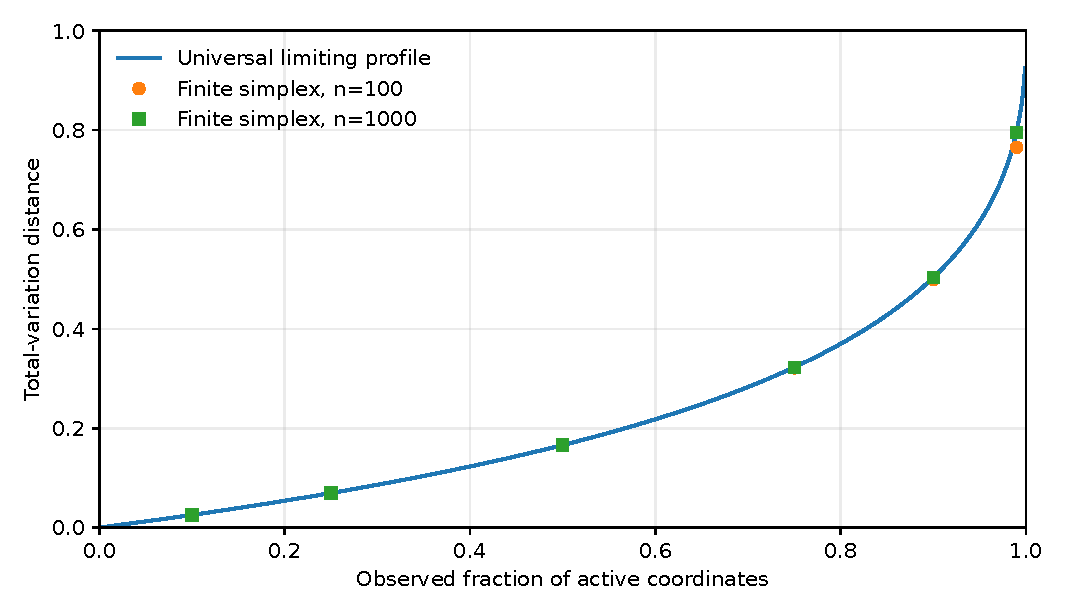
\includegraphics[width=.91\linewidth]{figures/tv_profile.pdf}
 \caption{The universal proportional-observation profile \eqref{eq:profile}.
 Markers are deterministic evaluations for the finite uniform-volume simplex
 proxy described in Section~\ref{sec:numerics}; they are not exact Fabius values.}
 \label{fig:profile}
\end{figure}

\begin{corollary}[Local independence versus global information]
\label{cor:globalinfo}
For the full configuration,
\begin{equation}
 \TV(P_x,Q_t)\longrightarrow1,\qquad
 \KL(P_x\Vert Q_t)=\frac12\log(2\pi n)-1+o(1).
 \label{eq:fullentropy}
\end{equation}
Nevertheless every observation mask with negligible tilted variance has
vanishing total-variation distance from its independent tilted law.
\end{corollary}
\begin{proof}
The total-variation assertion is the full-mask case of
Theorem~\ref{thm:mask}. From \eqref{eq:weight},
\[
 \KL(P_x\Vert Q_t)=-\EE_{P_x}H-\log D_t.
\]
Corollary~\ref{cor:slack} gives $\EE_{P_x}H\to1$, and
\eqref{eq:normalizer} gives the logarithmic term. The final assertion restates
\eqref{eq:variancecriterion}.
\end{proof}

The theorem shows why a fixed-dimensional Gibbs-conditioning principle alone
is incomplete here. It does not identify the largest admissible observation
scale, the nonzero proportional-block discrepancy, or the information still
present in the full configuration.

\section{A Brownian bridge for the active coordinates}
\label{sec:process}

Define a continuous process by linear interpolation of the values
\begin{equation}
 B_t(j/n)=\frac1{\sqrt n}\sum_{i=1}^j\big(Y_i-m(a_i)\big),
 \qquad j=0,\ldots,n.
 \label{eq:process}
\end{equation}
The indexing is by the number of active coordinates, not by their original
weights. Exponential tilting is what makes that indexing asymptotically
homogeneous.

\begin{theorem}[Conditioning turns Brownian motion into a bridge]
\label{thm:bridge}
As random elements of $C([0,1])$ with the uniform topology,
\begin{equation}
 B_t\Rightarrow B^0\quad\text{under }P_x,
 \qquad
 B_t\Rightarrow B\quad\text{under }Q_t,
 \label{eq:bridge}
\end{equation}
where $B$ is standard Brownian motion and
$B^0(u)=B(u)-uB(1)$ is a standard Brownian bridge. In particular,
\[
 \Cov(B^0(u),B^0(v))=\min(u,v)-uv.
\]
The conditioned bridge limit is jointly independent of the limiting
exponential slack. In the geometric case it is also jointly independent of
every fixed moving boundary window described in
Theorem~\ref{thm:boundary}.
\end{theorem}
\begin{proof}
Use Theorem~\ref{thm:global}, and represent the Dirichlet proportions as
$D_i=E_i/G_N$, where the $E_i$ are independent $\Exp(1)$ variables,
$G_N=\sum_{i\le N}E_i$, and these auxiliary variables are independent of the
model tail and slack. Let $L_N$ be the linearly interpolated centered partial
sum process of the $E_i$, divided by $\sqrt N$.

The elementary exponential invariance principle gives $L_N\Rightarrow B$;
a proof is included in Appendix~\ref{app:invariance}. The linearly interpolated
Dirichlet cumulative process satisfies the exact identity
\begin{equation}
 \sqrt N\left(\sum_{i\le Nu}^{\mathrm{interp}}D_i-u\right)
 =\frac{N}{G_N}\big(L_N(u)-uL_N(1)\big).
 \label{eq:dirbridge}
\end{equation}
Since $G_N/N\to1$ in probability, it converges to $B^0$.

In the global model, on the event of positive radius,
\[
 A-N=-W-E-\eps=O_P(\sqrt{\ell+1}).
\]
The exceptional nonpositive-radius event tends to zero. Thus
$(A-N)/\sqrt n\to0$ and $A/N\to1$ in probability. Multiplying the Dirichlet
process by the radius and centering the first $N$ coordinates by $m(a_i)$
instead of one changes the bulk process by a term tending uniformly to zero:
the radial error is at most $|A-N|/\sqrt n$, and the total centering discrepancy
is at most $\eps/\sqrt n$.

For the last $\ell$ active coordinates, the maximum absolute cumulative
contribution after centering is at most $(R+r)/\sqrt n$. Under the model this
is $O_P((\ell+1)/\sqrt n)=o_P(1)$, by Lemma~\ref{lem:tail}. Also $N/n\to1$,
so the change from the bulk time scale $j/N$ to $j/n$ disappears in the uniform
process limit. Total-variation contraction transfers the conclusion from the
model to $P_x$.

Under $Q_t$, couple the first $N$ coordinates to independent exponentials
with failure probability at most $\delta$, and use the same tail and centering
bounds. This gives the Brownian-motion assertion.

Finally, the Dirichlet process in \eqref{eq:dirbridge} is a function of the
proportions alone and is independent, for each $t$, of the model slack and
tail. Its radial approximation error vanishes in probability. Product weak
convergence therefore proves the stated joint independence, once the finite
boundary-window convergence is established below.
\end{proof}

This process theorem explains the proportional-block likelihood profile.
An observed fraction $\alpha$ of the active sum has asymptotic conditional
variance $\alpha(1-\alpha)$ rather than the tilted variance $\alpha$.
The Gaussian density ratio in \eqref{eq:likelihoodlimit} records exactly
that reduction. The full path theorem is stronger than this explanation:
it also controls all partial sums simultaneously.

\section{Geometric weights: a microscopic phase that does not disappear}
\label{sec:phase}

Take $w_j=b^{-j}$ with $b>1$. Then
\begin{equation}
 n=\lfloor\log_b t\rfloor,\qquad
 \theta=\{\log_b t\},\qquad
 a_{n+r}=b^{\theta-r}.
 \label{eq:phase}
\end{equation}
At indices well before $n$, the caps diverge and the exponential description
applies. Near $n$, the caps remain of order one and retain the phase $\theta$.

\begin{theorem}[Phase-dependent boundary law]
\label{thm:boundary}
Let $J\subset\ZZ$ be finite. Along any sequence with
$\theta\to\theta_0\in[0,1]$, the conditioned boundary window satisfies
\begin{equation}
 \Law_{P_x}\big((Y_{n+r})_{r\in J},H\big)
 \longrightarrow
 \left(\bigotimes_{r\in J}p_{b^{\theta_0-r}}(y_r)\,dy_r\right)
 \otimes\Exp(1)
 \quad\text{in total variation}.
 \label{eq:boundary}
\end{equation}
For the original uniforms $U_{n+r}$ the limiting density on $[0,1]$ is
\begin{equation}
 u\longmapsto
 \frac{a e^{-au}}{1-e^{-a}},\qquad a=b^{\theta_0-r}.
 \label{eq:boundaryU}
\end{equation}
The convergence is joint with the bridge in Theorem~\ref{thm:bridge}, in the
product of the uniform process topology and the finite-dimensional topology;
all the displayed limiting components are independent.
\end{theorem}
\begin{proof}
Since $\ell\to\infty$, every fixed index $n+r$ belongs to the tail beyond
$N=n-\ell$ for all sufficiently large $n$. The global approximation therefore
compares the boundary window and slack, with error $O_b(\rho_n)$, to their
independent tilted laws. Formula \eqref{eq:phase} gives the exact cap of each
coordinate. The truncated-exponential density depends continuously in $L^1$
on its positive cap, so these tilted laws converge in total variation.
For the original uniforms the same argument uses their exact tilted densities
$a e^{-au}/(1-e^{-a})$ on a common interval $[0,1]$. The process independence
was proved by the product construction in Theorem~\ref{thm:bridge}.
\end{proof}

The endpoint $\theta_0=1$ denotes a limit from below; the fractional part
itself lies in $[0,1)$. At the phase reset, the definition of $n$ shifts by
one. Thus the laws at phases zero and one are related by a relabeling, not
by equality at a fixed offset $r$.

There is no phase-independent limit for $U_n$ as $x\downarrow0$ without
subsequence selection. For a uniform variable tilted by $e^{-au}$, its mean
has derivative $-\Var(U)<0$ with respect to $a$. Hence the distributions in
\eqref{eq:boundaryU} at, for example, $a=1$ and $a=b^{1/2}$ differ. Both
phases are realized by taking $t=b^{m+\theta_0}$ and choosing $x$ from the
saddle equation. This is an order-one microscopic effect, despite the
phase-free Gaussian and exponential macroscopic limits.

\begin{figure}[t]
 \centering
 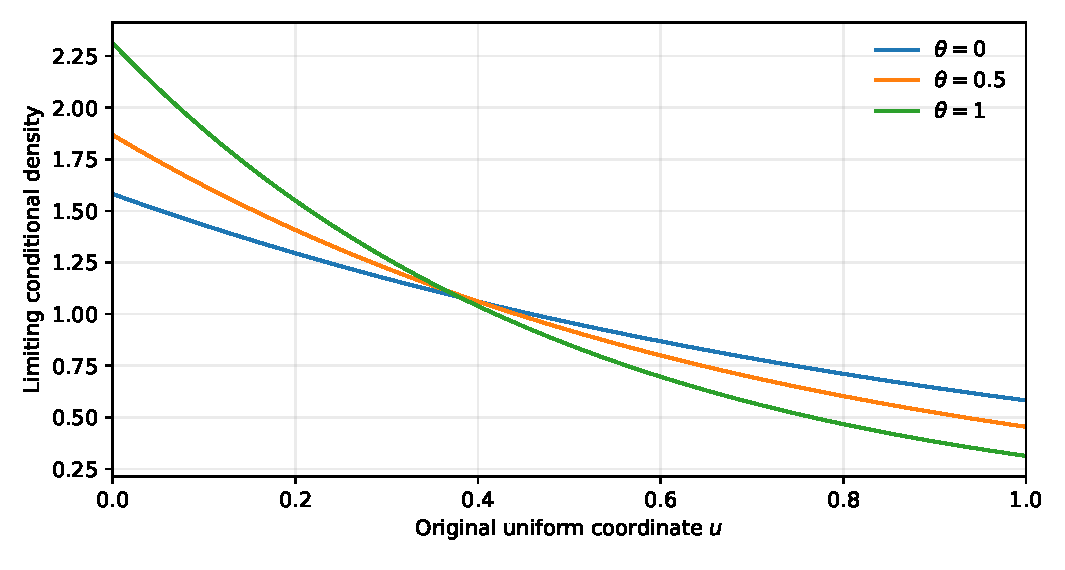
\includegraphics[width=.88\linewidth]{figures/boundary_phase.pdf}
 \caption{Dyadic boundary densities for $U_n$, with limiting phase
 $\theta=0,1/2,1$. The phase-one curve is a limit from below, before the
 active-index reset. The formula is \eqref{eq:boundaryU}, with $a=2^\theta$.}
 \label{fig:boundary}
\end{figure}

\subsection{An exact phase decomposition of the effective mean}

It is useful to distinguish a periodic correction from an index-dependent
one. Define, for real $\theta$,
\begin{equation}
 \kappa_b(\theta)=
 \sum_{r\le0}\big(m(b^{\theta-r})-1\big)
 +\sum_{r\ge1}m(b^{\theta-r}).
 \label{eq:kappa}
\end{equation}
Both sums converge locally uniformly, by exponential decay on the left and
geometric decay on the right. From the exact index range $r\ge1-n$,
\begin{equation}
 \mu=n+\kappa_b(\theta)+O_b(te^{-t}).
 \label{eq:muphase}
\end{equation}
Shifting the summation index gives
\[
 \kappa_b(\theta+1)=\kappa_b(\theta)+1.
\]
Consequently $\kappa_b$ itself is \emph{not} one-periodic. The continuous
one-periodic correction is
\[
 \eta_b(\theta)=\kappa_b(\theta)-\theta,
 \qquad
 \mu=\log_b t+\eta_b(\log_b t)+O_b(te^{-t}).
\]
Here $\eta_b$ is extended periodically. An analogous formula holds for $V$
with $m$ replaced by $v$ and error $O_b(t^2e^{-t})$. We do not need, and do
not assert here, a nonvanishing Fourier coefficient for these particular
phase functions. The nonconstant boundary densities already prove the
microscopic phase effect directly.

\subsection{Translation to the small endpoint parameter}

From $tx=n+O_b(1)$ and $\log_b t=n+\theta$,
\begin{equation}
 n=\log_b(1/x)+\log_b\log_b(1/x)+O_b(1),\qquad
 t\sim\frac{\log(1/x)}{x\log b}.
 \label{eq:xtoN}
\end{equation}
To see this, write
$\log_b t=\log_b(1/x)+\log_b(n+O_b(1))$.
It first gives $n/\log_b(1/x)\to1$, and reinsertion gives the displayed
second term. Thus the slack scale is approximately
$x\log b/\log(1/x)$, much smaller than $x$ itself. The number of active
coordinates is approximately logarithmic in $1/x$.

For $b=2$, \eqref{eq:fabius} is the Fabius distribution in its increasing
$[0,1]$ normalization. One can check the scale without any special-function
identity: $S_2$ has the distribution of $(U+S_2')/2$, with $U$ independent
of a copy $S_2'$. Thus
\[
 F_2(x)=\int_0^1 F_2(2x-u)\,du,
\]
where $F_2=0$ below zero and $F_2=1$ above one. Differentiation gives
$F_2'(x)=2F_2(2x)$ for $0<x<1/2$, and $F_2(1)=1$.

\section{Extremes, empirical laws, and examples beyond the dyadic case}
\label{sec:extreme}

\begin{theorem}[A Gumbel maximum and an exponential empirical law]
\label{thm:extremes}
Under $P_x$,
\begin{equation}
 \max_{j\ge1}Y_j-\log n\Rightarrow G,
 \qquad P(G\le z)=\exp(-e^{-z}).
 \label{eq:gumbel}
\end{equation}
For every bounded Lipschitz function $f:[0,\infty)\to\RR$,
\begin{equation}
 \frac1n\sum_{j=1}^n f(Y_j)
 \longrightarrow\int_0^\infty f(y)e^{-y}dy
 \quad\text{in }P_x\text{-probability}.
 \label{eq:empirical}
\end{equation}
The maximum limit is jointly independent of the limiting slack and, in the
geometric case, a fixed moving boundary window.
\end{theorem}
\begin{proof}
Work first in the global model. With $D_i=E_i/G_N$,
\[
 \max_{j\le N}Y_j^*=(A/G_N)\max_{i\le N}E_i.
\]
We have $A/G_N=1+O_P(N^{-1/2})+O_P(\sqrt{\ell+1}/N)$, and
$\max_{i\le N}E_i=\log N+O_P(1)$. Therefore replacing the factor $A/G_N$
by one changes the centered maximum by $o_P(1)$. The elementary identity
\[
 P\big(\max_{i\le N}E_i-\log N\le z\big)
 =\big(1-e^{-z}/N\big)^N
\]
for sufficiently large $N$ proves the Gumbel limit for the bulk.

For the tail, put $h_n=\log n+z$, which eventually exceeds one. Coordinates
$j>n$ have caps below one and cannot exceed $h_n$. There are only $\ell$
remaining active tail coordinates, and each has tilted exceedance probability
at most $2e^{-h_n}$ whenever its cap is at least $h_n$; otherwise the probability
is zero. Hence
\[
 Q_t^{>N}\big(\max_{j>N}Y_j>\log n+z\big)
 \le2\ell e^{-z}/n\longrightarrow0.
\]
Together with $\log N-\log n\to0$ and the global total-variation bound, this
proves \eqref{eq:gumbel}.

For \eqref{eq:empirical}, the first $N$ model coordinates are $cE_i$ with
$c=A/G_N\to1$ in probability. Their average difference under a Lipschitz
function is bounded by
\[
 \frac{\operatorname{Lip}(f)}{N}|c-1|\sum_{i\le N}E_i=o_P(1).
\]
The ordinary law of large numbers for $f(E_i)$ applies. The remaining
$\ell=o(n)$ terms have a bounded contribution because $f$ is bounded.

For joint independence, use $N\max_i D_i-\log N$, a function of the
Dirichlet proportions alone. It has the same Gumbel limit and differs from
the radius-rescaled bulk maximum by $o_P(1)$. The proportions are independent
of the model slack and tail for every $t$. Product convergence and
Theorem~\ref{thm:global} finish the proof.
\end{proof}

We have not used or asserted independence between the limiting bridge and
the limiting maximum. That stronger joint assertion is a natural extension;
it is not necessary for any theorem in this manuscript.

\subsection{Three concrete consequences}

\paragraph{Observing half the active coordinates.}
Whether one observes an initial half-block, every other active coordinate,
or an arbitrary half of them together with all the inactive tail, the limiting
distance from the corresponding independent tilted law is
\[
 \vp(1/2)=0.16606407498\ldots,
 \qquad
 \ip(1/2)=\tfrac12(\log2-1/2)=0.09657359028\ldots.
\]
The vanishing $-1/n$ pair covariance does not imply joint independence of a
linear-size block.

\paragraph{Observing infinitely many harmless coordinates.}
Take $I_t=\{j>n\}$. This is an infinite set, but its total tilted variance is
$O_q(1)$, so \eqref{eq:variancecriterion} gives
$\TV(P_x^{I_t},Q_t^{I_t})\to0$. The relevant quantity is variance fraction,
not cardinality of the observed set.

\paragraph{Supergeometric weights.}
For $w_j=2^{-j^2}$, the ratio condition holds, for example, with $q=1/2$.
Now $n=\lfloor\sqrt{\log_2t}\rfloor$, and $tx=n+O(1)$ gives
\[
 n\sim\sqrt{\log_2(1/x)},\qquad
 t\sim\frac{\sqrt{\log_2(1/x)}}{x}.
\]
All the global, mask, bridge, and extreme-value theorems still apply, although
the number of observable almost-independent coordinates is much smaller
than in the Fabius case. A fixed geometric phase is not needed for those
theorems. The boundary-window formula, in contrast, specifically uses geometric
weights and is not silently extended to this example.

\section{Reproducible numerical checks}
\label{sec:numerics}

The package contains \texttt{verification.py}, the generated JSON and CSV data,
and both figure sources as PDF and PNG images. The computations use floating
point; they are not interval-certified inequalities and are not substitutes
for the proofs. Two distinct experiments are kept separate.

\subsection{An exactly specified finite simplex proxy}

Let $(X_1,\ldots,X_N)$ be uniform on the volume simplex
\[
 \{x_i\ge0:\ x_1+\cdots+x_N\le N\}.
\]
For $1\le k<N$, its first $k$ coordinates have likelihood relative to
$\Exp(1)^{\otimes k}$
\begin{equation}
 r_{N,k}(s)=\frac{N!}{(N-k)!N^k}
 e^s(1-s/N)^{N-k}\ind_{\{0\le s<N\}}.
 \label{eq:finiteproxy}
\end{equation}
This is a finite proxy, \emph{not} the exact finite truncation of the Fabius
conditioning problem. It has the same universal first correction and
proportional-block limit, and it is directly computable without Monte Carlo.

The sum $s/N$ under this simplex law has distribution
$\operatorname{Beta}(k,N-k+1)$, whereas $s$ under the reference product has
$\operatorname{Gamma}(k,1)$ distribution. The logarithm of
\eqref{eq:finiteproxy} is concave and has its maximum at $s=k$. Let $s_-$
and $s_+$ be the two endpoints of the interval where the likelihood is above
one; $s_-=0$ for $k=1$. Then the total-variation distance is the beta
probability of $[s_-/N,s_+/N]$ minus the gamma probability of $[s_-,s_+]$.
The script locates the endpoints by a bracketing solver, using the stable
constant
\[
 \log\frac{N!}{(N-k)!N^k}=\sum_{j=0}^{k-1}\log(1-j/N).
\]
Thus the calculation evaluates an exact distributional formula numerically,
rather than estimating a high-dimensional density by sampling.

\begin{table}[htbp]
\centering
\caption{Finite simplex distances and the universal limiting profile.}
\label{tab:tv}
\begin{tabular}{rrrr}
\toprule
$\alpha=k/N$ & $N=100$ & $N=1000$ & $\vp(\alpha)$\\
\midrule
0.10 & 0.025593 & 0.025498 & 0.025488\\
0.25 & 0.069509 & 0.069492 & 0.069491\\
0.50 & 0.165814 & 0.166039 & 0.166064\\
0.75 & 0.321531 & 0.322560 & 0.322675\\
0.90 & 0.499380 & 0.502893 & 0.503283\\
0.99 & 0.765440 & 0.794850 & 0.798216\\
\bottomrule
\end{tabular}
\end{table}

For one coordinate, the values of $N\TV$ at
$N=100,1000,10000$ are respectively
$0.27157582$, $0.27076082$, and $0.27067959$; their limit is
$2e^{-2}=0.27067057\ldots$. This checks the factor of two in our
half-$L^1$ convention and the fixed-coordinate coefficient independently
of a simulation of the infinite series.

\subsection{Direct tilted importance sampling for the dyadic series}

For $n\in\{32,64,128,256\}$, the script takes $t=2^{n+0.37}$ and computes
the corresponding $x=\mu/t$. It samples the independent tilted coordinates
through index $n+50$ by the inverse distribution formula
\begin{equation}
 Y_j=-\log\big(1-V_j(1-e^{-a_j})\big),\qquad
 V_j\sim\operatorname{Unif}[0,1].
 \label{eq:sampler}
\end{equation}
The omitted scaled tail has deterministic upper bound
$2^{0.37-50}<1.2\cdot10^{-15}$. With $H=\mu-\sum_jY_j$ on the sampled
truncation, the nonnegative importance weight is
$e^{-H}\ind_{H\ge0}$. Weighted ratios estimate the conditioned expectations.
There are $240{,}000$ draws at each $n$, with seeds $20260928+n$.

The standard errors in Table~\ref{tab:mc} are ordinary importance-sampling
standard-error estimates. They describe sampling variability, not finite-$n$
asymptotic error or a rigorous confidence guarantee. In particular the last
row gives limiting targets, not the exact expectations at the sampled values
of $n$.

\begin{table}[htbp]
\centering
\small
\caption{Dyadic importance-sampling checks: estimate $\pm$ one estimated
Monte Carlo standard error. The midpoint process is defined in
\eqref{eq:process}.}
\label{tab:mc}
\begin{tabular}{rccc}
\toprule
$n$ & $D_t\sqrt{2\pi n}$ & $\EE_{P_x}H$ & $\EE_{P_x}B_t(1/2)^2$\\
\midrule
32  & $1.0229\pm0.0051$ & $0.9685\pm0.0037$ & $0.2346\pm0.0017$\\
64  & $1.0083\pm0.0062$ & $0.9860\pm0.0045$ & $0.2398\pm0.0021$\\
128 & $0.9953\pm0.0074$ & $0.9972\pm0.0054$ & $0.2473\pm0.0026$\\
256 & $1.0066\pm0.0090$ & $0.9890\pm0.0064$ & $0.2500\pm0.0032$\\
\midrule
Limit & $1$ & $1$ & $1/4$\\
\bottomrule
\end{tabular}
\end{table}

The JSON output additionally reports the boundary-coordinate mean, the slack
survival probability at one, the centered-maximum distribution at zero, and
effective sample sizes. Finite-size effects are visible: the Gumbel
probability at zero is about $0.4012$ at $n=32$, compared with its limit
$e^{-1}\approx0.3679$. This is not hidden by labeling the limiting law an
exact finite-size prediction. The deterministic simplex tests pass the
script's stated numerical tolerances. The script also checks the polynomial
normalization and moment coefficients using exact rational and factorial
arithmetic. No formal proof assistant was run.

\section{Research questions suggested by the results}
\label{sec:questions}

The following problems are proposed as continuations of this manuscript.
They are not claimed to be previously published open problems unless a
separate source establishes that status.

\paragraph{Q1. Is the logarithmic-logarithmic loss necessary?}
The full-configuration error is $O_q((1+\log\log n)/n)$ because the removable-cap
cutoff leaves $\ell\asymp\log\log n$ coordinates with order-one moments.
Can a more accurate radial correction give $O_q(1/n)$ without losing an
explicit sampling description? A matching lower bound for the present model
would also be useful. One should distinguish optimal approximation of the
entire configuration from optimal approximation of a fixed marginal.

\paragraph{Q2. All-order conditional expansions and the first phase coefficient.}
The exact likelihood \eqref{eq:exactlikelihood} permits higher-order gamma
expansions. The first term is universal after expressing it in $n$ and the
scaled coordinates; tail variance cancels. Determine the full second-order
term, track the cutoff-independent combination of tail cumulants, and identify
where the geometric phase first enters. The repository's periodic saddle
coefficient infrastructure is a natural source of comparison, but phase
substitution must be justified rather than performed formally.

\paragraph{Q3. Power-law densities at the left endpoint.}
Replace the uniforms by independent variables with densities
$u^{\gamma-1}g_j(u)$ near zero, with $g_j(0)>0$ and suitable uniform regularity.
The tilted bulk should approach gamma variables of shape $\gamma$, with
Dirichlet$(\gamma,\ldots,\gamma)$ proportions. Establish a full-product coupling,
not just fixed-dimensional weak convergence. For varying shapes, determine
whether the sharp criterion is the observed fraction of total gamma shape.

\paragraph{Q4. Beyond uniform lacunarity.}
Weights with $w_{j+1}/w_j\to1$ may have a macroscopic transition region rather
than $O(1)$ boundary variance. Identify verifiable hypotheses under which a
variance-fraction threshold and Gaussian likelihood profile still hold.
Polynomial and stretched-exponential weights should be treated separately.
A proof must exclude domination by a few coordinates; an analogy with the
current active-count argument does not do so automatically.

\paragraph{Q5. Several constraints.}
Condition on several weighted sums simultaneously. Is there an explicit
analogue of the random simplex model, with a finite-rank Gaussian projection
in place of the Brownian bridge? Determine which covariance matrix replaces
$1-\alpha$ in the likelihood profile, and how independent exponential slacks
are modified when the conditioning region has intersecting faces.

\paragraph{Q6. The almost-full observation regime.}
Theorem~\ref{thm:mask} gives distance tending to one when the unobserved active
fraction vanishes, but it does not give a sharp rate if $n-k$ grows slowly
or stays bounded. Analyze the competition between the number of unobserved
bulk coordinates, the $\log\log n$ cutoff tail, and the order-one slack.
The endpoint expansion in \eqref{eq:profileends} alone does not justify an
interchange of the proportional and almost-full limits.

\paragraph{Q7. Point-process extremes and joint process limits.}
Prove convergence of the full extremal point process, with explicit rates,
and establish its joint independence from the Brownian bridge where valid.
The Dirichlet representation suggests a Poisson limit inherited from
exponential order statistics, but the common normalization and the infinite
tail must be controlled jointly. The present manuscript proves only the
maximum limit and its independence from slack and boundary windows.

\paragraph{Q8. Certified sampling and complexity.}
Turn the global approximation into a finite algorithm with an explicit
user-selected total-variation error. A geometric tail can be truncated with
a deterministic norm bound, but truncating coordinates is not automatically
small in total variation on the full product space. A correct algorithm must
specify its output representation, the observables it approximates, and the
metric in which the truncation is certified. Determine the runtime needed
for endpoint conditional quantiles or bounded observables.

\paragraph{Q9. Exact shells versus inequalities.}
Replace $S\le x$ by a narrow interval $x-h_t\le S\le x$, or by a regular
conditional law at $S=x$. Identify the transition as $th_t$ tends to zero,
a finite constant, or infinity. The exponential slack should be truncated
or collapse to zero in the appropriate regimes; the first fixed-coordinate
correction should change correspondingly. State the version of conditioning
on a null event explicitly.

\paragraph{Q10. Random weights and phase mixing.}
For random lacunary weights, establish quenched and annealed analogues.
Does averaging over a random multiplicative scale erase the geometric
boundary phase, and what mixture replaces \eqref{eq:boundaryU}? Such a
mixture is not the same as evaluating the phase-dependent density at an
average phase. Uniform constants in the deterministic coupling are a useful
starting point, but integrability of the random lacunarity parameter needs
its own analysis.

\paragraph{Q11. Formal verification of the conditioning layer.}
A practical first formalization target is the gamma disintegration and the
finite-dimensional $L^1$ expansion, not the full functional limit theorem.
One can then connect an infinite-product tilt, countable-product total
variation, and cap-removal lemmas to the existing Fabius probability model.
The correctness boundary should explicitly distinguish formal inequalities,
classical analytic facts imported from a library, and floating-point
experiments. No Lean source purporting to certify these new results is
included here.

\section{A proof-status ledger and conclusions}
\label{sec:status}

\begin{table}[htbp]
\centering
\small
\caption{Status of the principal components.}
\begin{tabular}{>{\raggedright\arraybackslash}p{.32\linewidth}>{\raggedright\arraybackslash}p{.59\linewidth}}
\toprule
Component & Status in this package\\
\midrule
Fabius random-series representation & Classical background, cited and normalization checked.\\
Finite exponential-family variation phenomenon & Classical provenance acknowledged; the needed gamma calculations are rederived.\\
Full lacunary configuration coupling & Proved in Theorem~\ref{thm:global}, under the explicit ratio assumption.\\
First marginal correction and mask criterion & Proved in Theorems~\ref{thm:correction} and \ref{thm:mask}; no formal certification claimed.\\
Bridge, slack, phase, and maximum & Proved with the stated modes of convergence and independence scopes.\\
Numerical tables & Reproducible floating-point checks, not proofs or rigorous error certificates.\\
Repository asymptotic audit & Inspected source report; its Lean build and axiom audit were not rerun.\\
Worldwide novelty / published open problem & No exhaustive priority determination and no claim to resolve a named published conjecture.\\
\bottomrule
\end{tabular}
\end{table}

The central conclusion is a distinction between three scales. A negligible
variance fraction is asymptotically unaffected by the global constraint after
exponential tilting. A positive fraction retains a universal, exactly
quantified dependence. The full configuration retains a logarithmically
growing relative-entropy cost and becomes maximally distinguishable from
the independent tilted product.

The simplex approximation explains all three scales without discarding the
infinite tail. For geometric weights it simultaneously separates universal
bulk behavior from a phase-dependent boundary layer. This is the proposed
addition to the repository's Fabius research program: a configuration-level
conditioning theory complementing scalar endpoint asymptotics.

\appendix
\section{An elementary exponential invariance principle}
\label{app:invariance}

Let $E_1,E_2,\ldots$ be independent $\Exp(1)$ variables, $X_i=E_i-1$, and
let $L_N$ linearly interpolate
$N^{-1/2}\sum_{i\le j}X_i$ at times $j/N$. We justify the fact
$L_N\Rightarrow B$ in $C([0,1])$ used in Theorem~\ref{thm:bridge}.

For finite-dimensional distributions, disjoint partial-sum increments are
independent. The characteristic function of $X_i$ satisfies
\[
 \EE e^{iuX_i}=1-u^2/2+O(|u|^3)\quad(u\to0).
\]
For a block of length $m_N$ with $m_N/N\to a$, its scaled characteristic
function tends to $e^{-au^2/2}$. Applying this to finitely many disjoint
blocks proves convergence to independent normal increments. Interpolation
at finitely many endpoints changes the random variables by $o_P(1)$,
since a single $X_i/\sqrt N$ tends to zero in probability.

For tightness, independence and the exponential moments give
\[
 \EE\left(\sum_i c_iX_i\right)^4
 =3\left(\sum_i c_i^2\right)^2+6\sum_i c_i^4.
\]
The increment $L_N(t)-L_N(s)$ has coefficients $c_i/\sqrt N$ with
$0\le c_i\le1$ and $\sum_i c_i=N(t-s)$. If $t-s\ge1/N$, then
$\sum_i c_i^2\le N(t-s)$ and $\sum_i c_i^4\le N(t-s)$; thus its fourth
moment is at most $C(t-s)^2$. If $t-s<1/N$, the sum of the coefficients
is at most one, so both terms in the displayed fourth-moment formula are
bounded by a constant times $N^4(t-s)^4$. After division by $N^2$ this
is again at most $C(t-s)^2$. We have proved uniformly in $N$ that
\[
 \EE|L_N(t)-L_N(s)|^4\le C|t-s|^2.
\]
The standard fourth-moment tightness criterion for continuous processes
therefore applies. To recall its mechanism, apply Markov's inequality to
dyadic increments, sum their probabilities over each dyadic level, and
choose a H\"older exponent below $1/4$; the resulting summable geometric
bound controls the modulus of continuity. Finite-dimensional convergence
then identifies the unique limit as standard Brownian motion.

\section{Reproduction and source record}
\label{app:reproduce}

The archive is self-contained for PDF compilation: the LaTeX source uses an
embedded bibliography and the included figure PDFs. No online source fetch is
performed by the build. A standard TeX Live installation with
\texttt{newtx}, \texttt{microtype}, and the usual AMS packages suffices.

\begin{verbatim}
pdflatex -interaction=nonstopmode -halt-on-error article.tex
pdflatex -interaction=nonstopmode -halt-on-error article.tex
python verification.py --draws 240000
\end{verbatim}

The numerical script requires Python 3.11 or later, NumPy, SciPy, and
Matplotlib. The delivered run used NumPy 2.3.5, SciPy 1.17.0, and
Matplotlib 3.10.8. The output includes all figures and
\texttt{data/verification\_results.json}. The optional
\texttt{--skip-monte-carlo} flag reruns only the deterministic simplex checks.
The \texttt{Makefile} provides equivalent build targets.

The repository snapshot was obtained from its recursive tree and the
asymptotic audit was read at the pinned commit. The bibliography points to
that pinned audit, rather than an unspecified future branch state. Narrow
repository searches for Gibbs conditioning and Brownian-bridge terminology
were used to choose a research direction, not to certify absence of overlap.
The cited 2026 version of Cator--Ferrari was checked on arXiv; the
Diaconis--Freedman comparison is supported by the publisher's abstract and
bibliographic record. The proofs here do not rely on an inaccessible theorem
statement from that paper.

\begin{thebibliography}{9}

\bibitem{arias}
J. Arias de Reyna,
\emph{An infinitely differentiable function with compact support:
Definition and properties}.
English translation of the original article in
Revista de la Real Academia de Ciencias Exactas, F\'isicas y Naturales
\textbf{76} (1982), 21--38.
\href{https://arxiv.org/abs/1702.05442}{arXiv:1702.05442} (2017).
Theorem~3 supplies the random-series interpretation used here.

\bibitem{df}
P. Diaconis and D. A. Freedman,
\emph{Conditional limit theorems for exponential families and finite versions
of de Finetti's theorem}.
Journal of Theoretical Probability \textbf{1} (1988), 381--410.
\href{https://doi.org/10.1007/BF01048727}{doi:10.1007/BF01048727}.

\bibitem{cf}
E. Cator and P. A. Ferrari,
\emph{Gibbs conditioning principle for log-concave independent random variables}.
Markov Processes and Related Fields \textbf{32} (2026), 63--77.
\href{https://arxiv.org/abs/2512.24910v3}{arXiv:2512.24910v3},
revised June 19, 2026.
\href{https://doi.org/10.61102/1024-2953-mprf.2026.32.1.00a}
{doi:10.61102/1024-2953-mprf.2026.32.1.00a}.

\bibitem{repo}
V. Reshetnikov, \emph{ProveIt},
\texttt{Analysis/FabiusFunction/docs/ASYMPTOTIC\_COMPLETION\_AUDIT.md}.
Inspected September 28, 2026, at commit
{\small\texttt{2cdcd74f3abcbbff7bd47c6c4265522395def609}}.
\href{https://github.com/VladimirReshetnikov/ProveIt/blob/2cdcd74f3abcbbff7bd47c6c4265522395def609/Analysis/FabiusFunction/docs/ASYMPTOTIC_COMPLETION_AUDIT.md}
{Pinned source on GitHub}.
The audit's formalization claims are reported as source claims, not as a
build or axiom audit performed for this manuscript.

\end{thebibliography}
\end{document}
